 Indefinite Causal Order has overlap with many topics in Quantum Physics such as Quantum gravity, Quantum foundations, Computer Science and it has emerged into a new field in itself.Indefinite causal structure is when there is, in general, no matter of fact as to whether the separation between two events is time-like or not.
 It was originated from Lucius Hardy as an idea to define how quantum gravity can be explored by combining few radical concepts of quantum theory and general relativity.The causal structure in which a quantum circuit is built is normally fixed. But general relativity introduces us to a concept of causality.The matrix depends on the configuration of objects in space and time and therefore, have a dynamical causal structure. Though Lucian Hardy did not introduce the concept along with examples, various studies later tried to formulate and fit the notion of non-causality and causal inequality in various fields and provide examples \cite{Abbott_2016}\cite{Branciard_2016}\cite{Oreshkov_2016}.
 Two popular examples of Indefinite Causal Order that emerged were,\\
 1. Quantum Switch - A control system based process\cite{chiribella_2009}.\\
 2. The Oreshkov Cosla Brukner Process - A hypothetical process without usage of control system.\cite{OCB_12}

In this chapter, we explain breifly about the OCB process and further extend the explanation of Quantum Switch process, and it's various applications in the field of Quantum Information.
\section{OCB process}
In everyday life and in classical physics, events are ordered in time: a cause can only influence an effect in its future not in its past. As a simple example, imagine a person, Alice, walking into a room and finding there a piece of paper. After reading what is written on the paper Alice erases the message and leaves her own message on the piece of paper. Another person, Bob, walks into the same room at some other time and does the same: he reads, erases and re-writes some message on the paper. If Bob enters the room after Alice, he will be able to read what she wrote; however Alice will not have a chance to know Bob's message. In this case, Alice's writing is the "cause" and what Bob reads the "effect". Each time the two repeat the procedure, only one will be able to read what the other wrote. Even if they don't have watches and don't know who enters the room first, they can deduce it by what they write and read on the paper. For example, Alice might write "Alice was here today", such that if Bob reads the message, he will know that he came to the room after her.\\
As long as only the laws of classical physics are allowed, the order of events is fixed: either Bob or Alice is first to enter the room and leave a message for the other person. When quantum mechanics enters into play, however, the picture may change drastically and the causal order of events could be in such a superposition. If - in our example - Alice and Bob have a quantum system instead of an ordinary piece of paper to write their messages on, they can end up in a situation where each of them can read a part of the message written by the other. Effectively, one has a superposition of two situations: "Alice enters the room first and leaves a message before Bob" and "Bob enters the room first and leaves a message before Alice".\\
Such a superposition, however, has not been considered in the standard formulation of quantum mechanics since the theory always assumes a definite causal order between events.But if we believe that quantum mechanics governs all phenomena, it is natural to expect that the order of events could also be indefinite, similarly to the location of a particle or its velocity.\\
Although the concept provides an important step towards understanding Indefinite causal order, it also suggests that it might not be a mandatory property of nature challenging us to find out where in nature we should look for superpositions of causal orders.
\begin{figure}[htp]
\centering
\fbox{
\subfigure[Alice's side]{\includegraphics[scale=0.1]{figures/img/Screenshot 2024-06-10 at 6.23.53 PM.jpeg}}
%\hfill
\qquad
\subfigure[Bob's side]{\includegraphics[scale=0.1]{figures/img/Screenshot 2024-06-10 at 6.25.39 PM.jpeg}}}
\caption{\footnotesize{Pictorial representation of the OCB process}}
\label{eval_theta_modW}
\end{figure}
\section{Quantum Switch}
 Around 2020, ICO started gaining popularity in the area of Quantum Information using a simple circuit called Quantum Switch.
To explain the working of a Quantum Switch, let us consider the coherent superposition of two completely positive trace preserving maps using an additional control qubit. When the control qubit is prepared in the state $\ket{0}$, operation $\mathcal{N}_i$ (corresponding Kraus $\lbrace K_i \rbrace$) will act after $\mathcal{N}_j$ (corresponding Kraus $\lbrace K_j \rbrace$) whereas when the control qubit is prepared in the state $\ket{1}$, operation $\mathcal{N}_j$ (corresponding Kraus $\lbrace K_j \rbrace$) will act on the target state after $\mathcal{N}_i$ (corresponding Kraus $\lbrace K_i \rbrace$). The joint Kraus operators for the path superposition becomes,
\begin{equation}
    W_{ij} = K_i.K_j \bigotimes \ket{0} \bra{0} + K_j.K_i \bigotimes \ket{1}\bra{1}.
\end{equation}
Let us now prepare the control qubit in the state
\begin{equation}
    \rho_c = \alpha\ket{0}\bra{0} \pm (1-\alpha) \ket{1}\bra{1}.
\end{equation}
The overall operation will look like
\begin{equation}
    S_{ij}(\rho \bigotimes \rho_c) = W_{ij} (\rho \bigotimes \rho_c) W_{ij}^\dagger.
\end{equation}
Finally, the control qubit is measured in the $\lbrace \ket{+}\bra{+}, \ket{-}\bra{-} \rbrace$ basis, and hence the effective evolution of the target state will become.
\begin{equation}
    \rho_{S} = \bra{\pm} S_{ij}(\rho \bigotimes \rho_c) \ket{\pm}.
\end{equation}

\section{Application of quantum switch on global unitary operation}

In this section, we briefly discuss the action of quantum switch as defined in the literature of quantum information theory and further illustrate the action of the same while the channels under consideration are global unitaries. Quantum switch is a higher-order map that takes two or more channels as inputs and then outputs the superposition of their orders based on the state of the control qubit. With a quantum switch, one can in principle control the action of the channel with an ancillary system, which is the control. As mentioned in the introduction, here also we consider two channels $\mathcal{N}_1$ and $\mathcal{N}_2$. When the state of the control qubit is $\ket{0}\bra{0}$, the channel $\mathcal{N}_2$ acts before the channel $\mathcal{N}_1$, the action on the system can be written mathematically as, $(\mathcal{N}_1 \circ \mathcal{N}_2) \rho_{AB}$. On the other hand, when the ancillary qubit is in state $\ket{1}\bra{1}$, the action of the channels on the system is given by, $(\mathcal{N}_2 \circ \mathcal{N}_1) \rho_{AB}$. Now we consider the superposition of these two situations to obtain the final switching action. \\
%The whole circuit is illustrated in Fig.[] for better understanding.

Now let us consider that the Kraus operators corresponding to the channels  $\mathcal{N}_1$ and $\mathcal{N}_2$ are given by, $\{K_{i}^{(1)}\}$ and $\{K_{j}^{(2)}\}$ respectively, with $\sum_i {K^{(1)}_i}^{\dagger} K^{(1)}_i = \mathcal{I}$ and $\sum_j {K^{(2)}_j}^{\dagger} K^{(2)}_j = \mathcal{I}$. Hence the joint Kraus operator representing the complete action of the switch can be written as, 
 \begin{equation}
    W_{ij} = K_{i}^{(1)} \cdot K_{j}^{(2)} \otimes \ket{0}\bra{0} + K_{j}^{(2)} \cdot K_{i}^{(1)} \otimes \ket{1}\bra{1}.
    \label{switch_Kraus}
\end{equation}
Hence the final joint system-ancilla state can be written as, 
\begin{equation}
    S(\mathcal{N}_1,\mathcal{N}_2)(\rho \otimes \rho_c) = \sum_{i,j} W_{ij}(\rho_{AB} \otimes \rho_c)W_{ij}^{\dagger}.
    \label{switchaction}
\end{equation}
Here, $\rho_c$ is the initial state of the control qubit. In the end, the control qubit is measured in the coherent basis i.e. $\{\ket{+},\ket{-}\}$ and the final state of the system is obtained corresponding to each outcome as, 
\begin{equation}
    \rho_f = \frac{1}{n}~ _c\langle\pm|S(\mathcal{N}_1,\mathcal{N}_2)(\rho_{AB} \otimes \rho_c)|\pm\rangle_c
    \label{FS}
\end{equation}
with $\ket{\pm}=\frac{1}{2}(\ket{0}\pm\ket{1})$ and $n$ is the constant for normalization. \\
\iffalse
 \begin{figure}[htp]
    \fbox{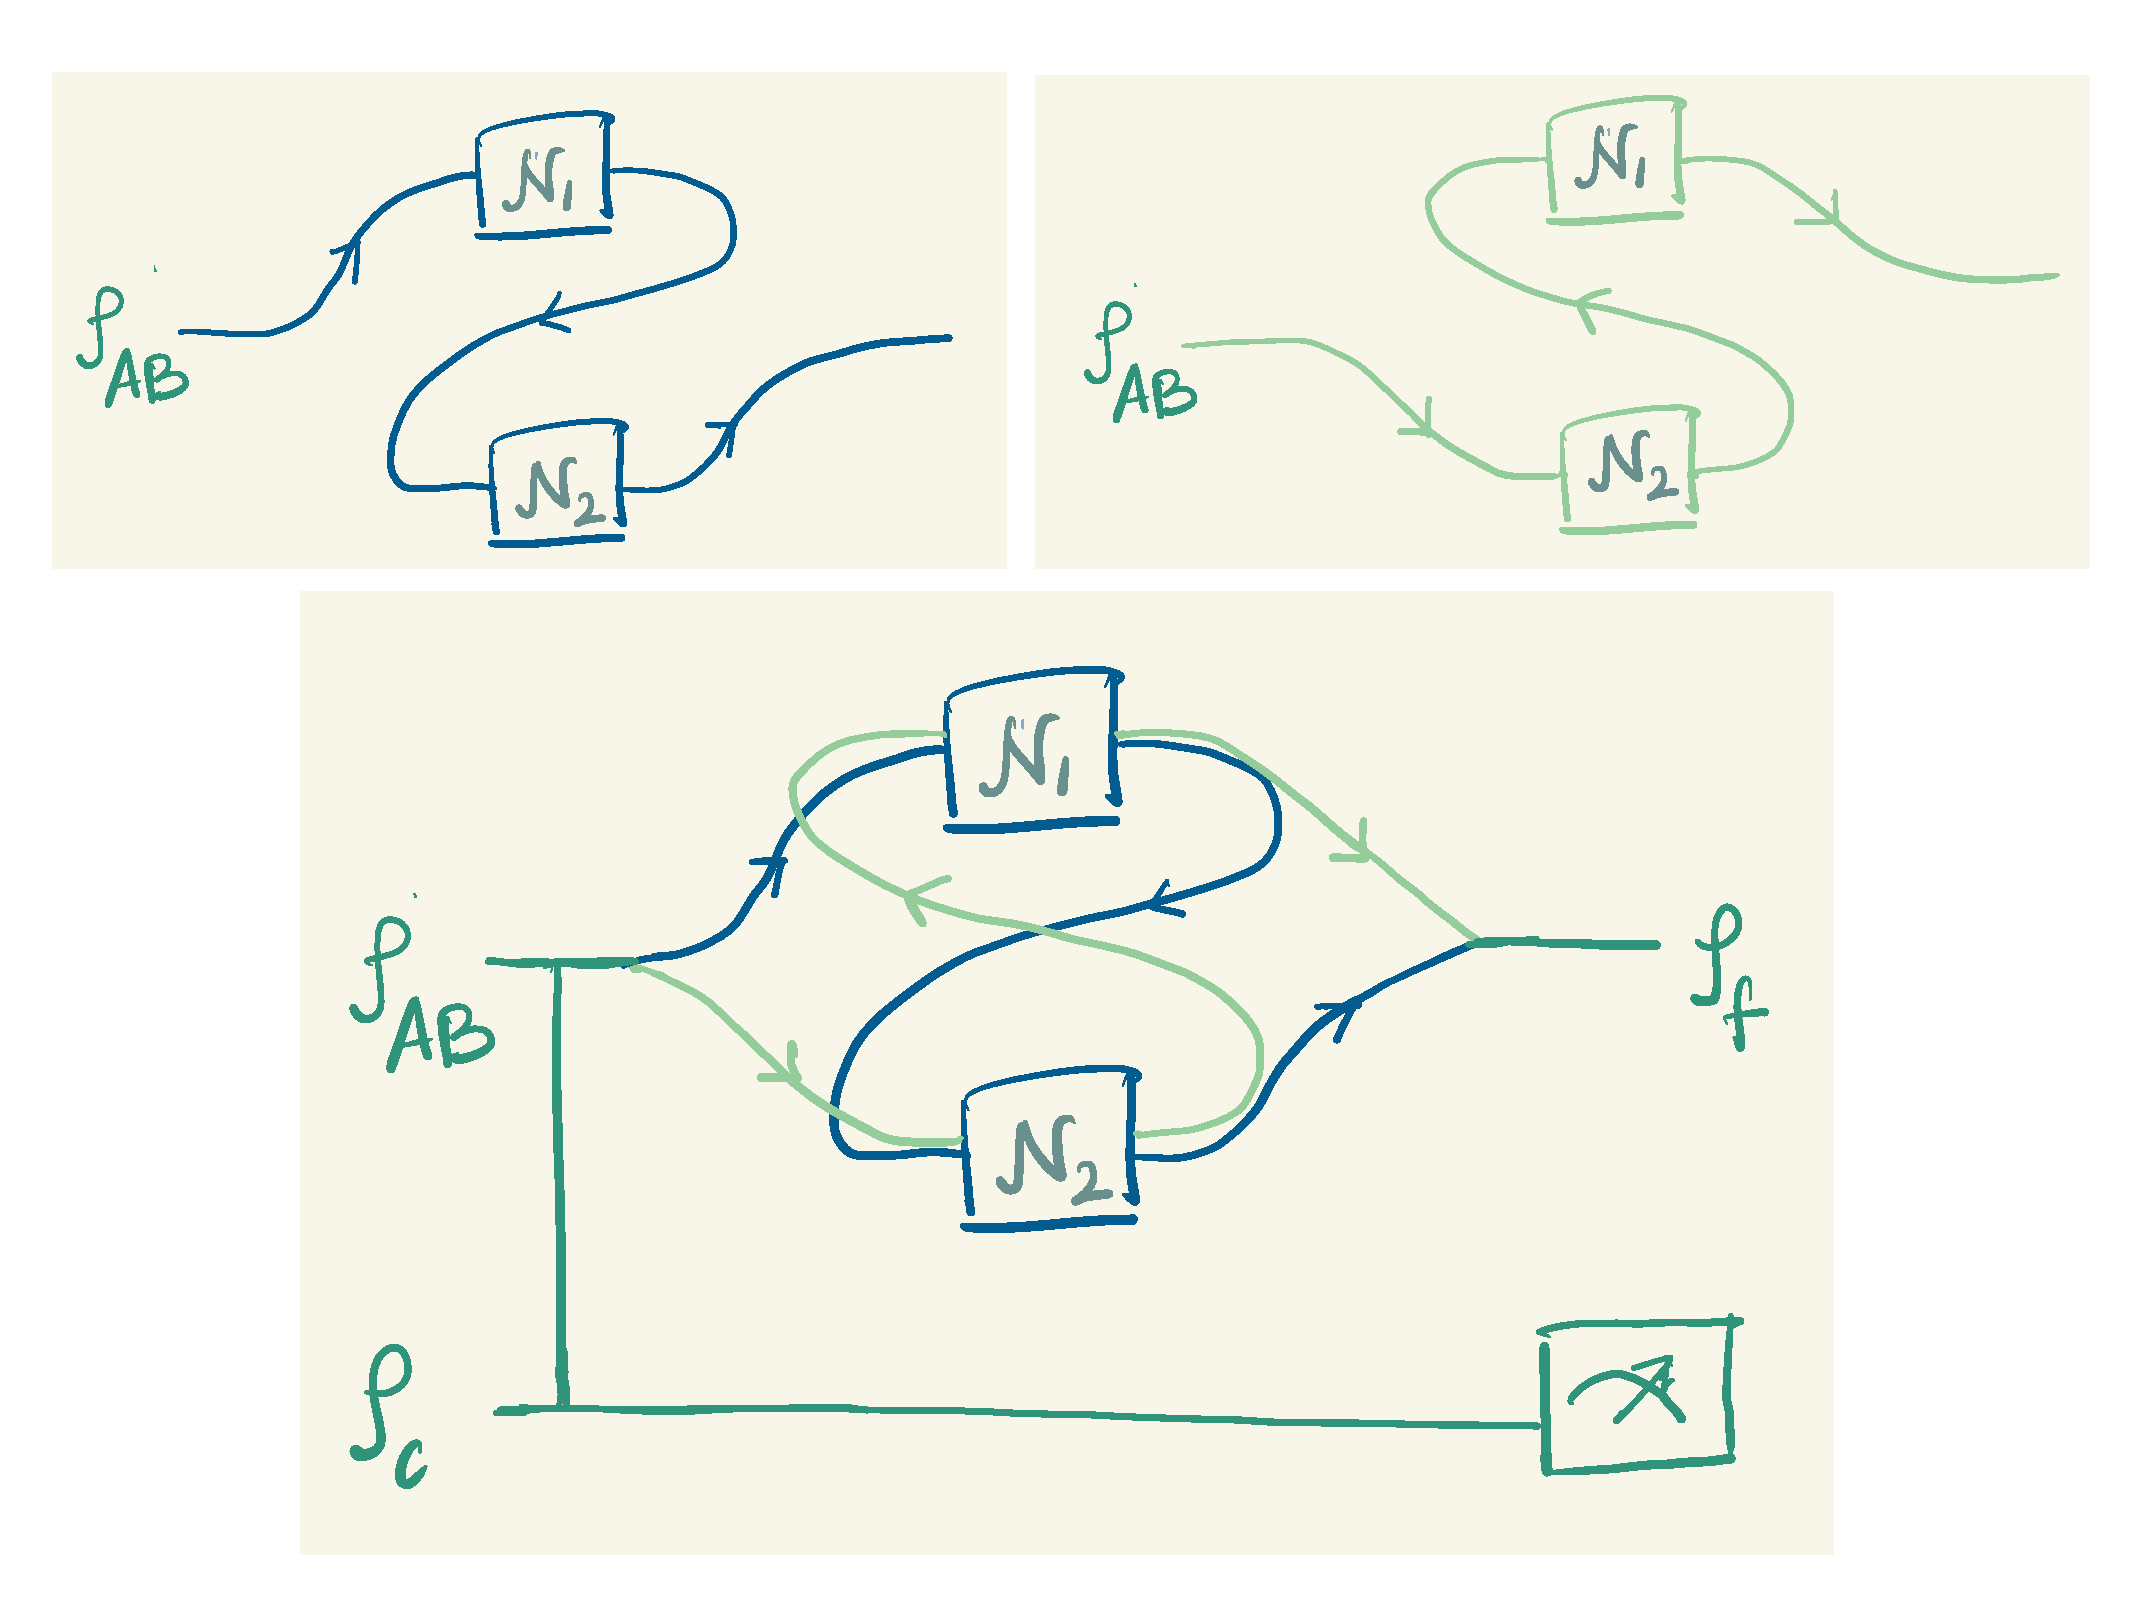
\includegraphics[scale=0.22]{switch_handdrawn_pic.pdf}}
    \caption{\footnotesize{Action of switch.}}
    \label{LHS_eval_cond_modW}
    \end{figure}
\fi

In our case, the two channels under consideration are two global unitary matrices acting on the bipartite system. Let the unitary matrices be $\mathcal{U}_1$ and $\mathcal{U}_2$ and hence the action of the switch can be simplified as given in the following.\\
\textit{The final state of the system after the measurement, considering both the control qubit and the projective measurement on the control qubit in the $\ket{+}$ basis becomes,
\begin{equation}
    \rho_f=\frac{\mathcal{L}_s \rho_{AB} \mathcal{L}_s^{\dagger}}{ Tr[\mathcal{L}_s \rho_{AB} \mathcal{L}_s^{\dagger}]}
    \label{finalstate_switch}
\end{equation}
where, the switching action of the unitary matrices can be seen as, $\mathcal{L}_s=\frac{1}{2}(\mathcal{U}_1 \mathcal{U}_2+\mathcal{U}_2 \mathcal{U}_1)$.}
%\label{prop2}

%\begin{proof}
    \noindent We give a proof of the above statement, particularly for our scenario. We begin by incorporating Eq. (\ref{switchaction}) into Eq. (\ref{FS}) to obtain,
    \begin{equation}
        \rho^{\prime}_{f} =~ _c\bra{+}\sum_{i,j} W_{ij}(\rho_{AB} \otimes \rho_c)W_{ij}^{\dagger}|\ket{+}_c.
    \end{equation}
    Evidently, $\rho_f= \rho^{\prime}_{f}/n$ with $n= Tr [\rho^{\prime}_{f}]$. Let us now simplify the preliminary calculation by considering that the initial state is given by $\rho_c=\ket{+}\bra{+}$. The calculation elaborated in the following is for the case when the control qubit is measured in the $\ket{+}$ state. Hence we have,
    \begin{eqnarray}
        \rho^{\prime}_{f} &=~& _c\bra{+} (\mathcal{U}_1 \mathcal{U}_2 \otimes \ket{0}\bra{0} + \mathcal{U}_2 \mathcal{U}_1 \otimes \ket{1}\bra{1}) \nonumber\\
        &&(\rho_{AB}\otimes \ket{+}\bra{+}) \nonumber\\
        &&(\mathcal{U}^{\dagger}_2 \mathcal{U}^{\dagger}_1 \otimes \ket{0}\bra{0} + \mathcal{U}^{\dagger}_1 \mathcal{U}^{\dagger}_2 \otimes \ket{1}\bra{1}) \ket{+}_c \nonumber\\
        %&=& (\mathcal{U}_1 \mathcal{U}_2 \rho_{AB} \mathcal{U}^{\dagger}_2 \mathcal{U}^{\dagger}_1) \vert \braket{0|+}\vert^4 \nonumber\\
        %&& (\mathcal{U}_1 \mathcal{U}_2 \rho_{AB} \mathcal{U}^{\dagger}_1 \mathcal{U}^{\dagger}_2) \vert \braket{0|+}\vert^2 \vert \braket{1|+}\vert^2 \nonumber\\
        %&& (\mathcal{U}_2 \mathcal{U}_1 \rho_{AB} \mathcal{U}^{\dagger}_2 \mathcal{U}^{\dagger}_1) \vert \braket{0|+}\vert^2 \vert \braket{1|+}\vert^2 \nonumber\\
        %&& (\mathcal{U}_2 \mathcal{U}_1 \rho_{AB} \mathcal{U}^{\dagger}_1 \mathcal{U}^{\dagger}_2) |\braket{1|+}|^4.
        &=& (\mathcal{U}_1 \mathcal{U}_2~|\braket{0|+}|^2 + \mathcal{U}_2 \mathcal{U}_1~|\braket{1|+}|^2 ) \rho_{AB} \nonumber\\
        && (\mathcal{U}^{\dagger}_2 \mathcal{U}^{\dagger}_1~ |\braket{0|+}|^2 + \mathcal{U}^{\dagger}_1 \mathcal{U}^{\dagger}_2~|\braket{1|+}|^2 ) \nonumber\\
        &=& \mathcal{L}_s \rho_{AB} \mathcal{L}^{\dagger}_s, 
    \end{eqnarray}
    with $\mathcal{L}_s=\frac{1}{2}(\mathcal{U}_1 \mathcal{U}_2+\mathcal{U}_2 \mathcal{U}_1)$. Now it is clear that $n=Tr[\mathcal{L}_s \rho_{AB} \mathcal{L}^{\dagger}_s]$ and the final state of the system after the switching action is given by the expression in Eq. (\ref{finalstate_switch}). Hence the claim.\\
The overall effect of switch can be seen by the operator $\mathcal{L}_s$. Note that, this is no more an unitary operation, which enables us to achieve the advantage in our case. 
